\documentclass[pdf]{beamer}
\mode<presentation>{}

\usepackage{multicol}
\usepackage{graphicx}
\usepackage{xcolor}
\usepackage{listings}
\usepackage{mips}
\usepackage{amsmath}
\usepackage{tikz}
\usepackage{url}
\usetikzlibrary{shapes,backgrounds,arrows, fit, positioning}
\usepackage{algpseudocode}


\definecolor{CommentGreen}{rgb}{0,.6,0}
\lstset{
 language=[mips]Assembler,
 escapechar=@, % include LaTeX code between `@' characters
 keepspaces,   % needed to preserve spacing with lstinline
 basicstyle=\footnotesize\ttfamily\bfseries,
 commentstyle=\color{CommentGreen},
 stringstyle=\color{cyan},
 showstringspaces=false,
 keywordstyle=[1]\color{blue},    % instructions
 keywordstyle=[2]\color{magenta}, % directives
 keywordstyle=[3]\color{red},     % registers
 }
 
\lstset{language=[mips]Assembler}

%% preamble
\title{Tamarin: Concolic Disequivalence for MIPS}

\author{Abel Nieto}
\date{}

\newcommand{\crule}[3][black]{\textcolor{#1}{\rule{#2}{#3}}}

\begin{document}

\begin{frame}
\titlepage
\end{frame}

\begin{frame}{A Tale of Two Boxes}
~\\
\crule{3cm}{3cm} \hspace{2cm} \crule{3cm}{3cm}
\end{frame}

\begin{frame}{A Tale of Two Boxes}
\hspace{3.5cm}\fbox{\includegraphics[width=1cm]{carrot}}
\\
\crule{3cm}{3cm} \hspace{2cm} \crule{3cm}{3cm}
\pause
\\
nom nom
\pause
\hspace{3.5cm}
nom nom
\pause
\\
\hspace{3.5cm}
{\Huge $=$}
\end{frame}

\begin{frame}{A Tale of Two Boxes}
~\\
\fbox{\includegraphics[width=3cmcm]{camel}} \hspace{2cm} \fbox{\includegraphics[width=3cm]{beaver}}
\\
\hspace{5cm} {\Huge $\neq$}
\end{frame}

\Large

\begin{frame}{The Problem}
Given MIPS program $P_1$ and $P_2$, when are they equivalent?
\end{frame}

\begin{frame}{The Problem}
Attempt 1: two programs are equivalent if they give the same output (resp.) for all inputs.
\pause
\\~\\
What's an input?
\pause
Register $\$1$ and $\$2$.
\pause
\\
What's an output?
\pause
Register $\$3$. 
\pause
\\~\\
Don't care about (most) CPU interrupts/IO.
\end{frame}

\begin{frame}{The Problem}
Attempt 1: two programs are equivalent if they give the same output (resp.) for all inputs.
\pause
\\~\\
Problem: undecidable via Rice's theorem.
\end{frame}

\begin{frame}[fragile]{The Problem}
Attempt 2: two programs are $S$-equivalent if they cannot be told apart after $S$ steps.
\pause
\\~\\
$S$-equivalent (e.g. for $S = 10$), but not equivalent:
\begin{multicols}{2}
\begin{lstlisting}[escapeinside={(*}{*)}]
# P_1
add $3, $1, $2
\end{lstlisting}
\vfill\null
\columnbreak
\begin{lstlisting}
# P_2
  add $4, $0, 1  # counter
  add $5, $0, 42 # upper bound
loop:
  slt $6, $4, $5 
  beq $6, $0, end
  add $4, $4, 1
  beq $0, $0, loop
end:
  add $3, $1, $1  
\end{lstlisting}
\end{multicols}
\end{frame}

\begin{frame}{The Problem}
Attempt 2: two programs are $S$-equivalent if they \textbf{cannot be told apart} after $S$ steps.
\vspace{1cm}

\begin{tabular}{l | l | l}
$R_1$ & $R_2$ & $S$-equiv \\
\hline
\pause
$v$ & $v$ & yes \\
\pause
$v$ & $w \neq v$ & no \\
\pause
$v$ & error & no \\
\pause
error & error & yes \\
\pause
non-termination & ??? & yes \\
$\ldots$

\end{tabular}
\end{frame}

\begin{frame}{The Problem}
\begin{lemma}
Equivalence implies $S$-equivalence.
\end{lemma}

\pause
~\\
\begin{corollary}[Soundness]
If two programs are not $S$-equivalent (for any $S$), then they are not equivalent.
\end{corollary}
\end{frame}

\begin{frame}{The Problem}
Attempt 2: two programs are $S$-equivalent if they \textbf{cannot be told apart} after $S$ steps.
\\~\\
Which inputs?
\pause 
\\~\\
Try some inputs by hand: low coverage, fast (unit tests)
\pause
\\~\\
Try all $2^{64}$values of $\$1$ and $\$2$: high coverage, slow (but decidable)
\pause
\\~\\
\textbf{Tamarin}: use concolic execution: higher coverage(?), not too slow(?)
\end{frame}

\begin{frame}[fragile]{Idea}

Alternating concolic execution

\begin{multicols}{2}
\begin{lstlisting}[escapeinside={(*}{*)}]
# P_1
  bne $1, 42, end
  add $3, $3, $0
end:
  add $3, $1, $2
\end{lstlisting}
\vfill\null
\columnbreak
\begin{lstlisting}
# P_2
  add $3, $1, $2  
  bne $2, 100, end
  add $3, $3, $2
end:
\end{lstlisting}
\end{multicols}

\pause

\begin{tabular}{l | l | l | l | l | l | l | l}
Run & Driver & Verifier & $\$1$ & $\$2$ & Path & $R_D$ & $R_V$ \\
\hline
\pause
1 & $P_1$ & $P_2$ & 1 & 1 & $\$1 \neq 42$ & 2 & 2 \\
\pause
2 & $P_2$ & $P_1$ & 1 & 1 & $\$2 \neq 100$ & 2 & 2\\
\pause
3 & $P_1$ & $P_2$ & 42 & 1 & $\$1 = 42$ & 2 & 2 \\
\pause
4 & $P_2$ & $P_1$ & 1 & 100 & $\$2 = 100$ & \textcolor{red}{201} & \textcolor{red}{2}
\end{tabular}
\end{frame}

\begin{frame}{Tamarin (Overview)}
\normalsize

\begin{tikzpicture}[remember picture,overlay]

\node [draw] at (5,0) (tam) {Tamarin};
\node at (2, 0.5) (p1) {$P_1$};
\node at (2, -0.5) (p2) {$P_2$};


\draw [-latex] (p1) -- (tam);
\draw [-latex] (p2) -- (tam);
\pause
\node at (9, 0.5) (equiv) {$S$-equivalent};
\draw [-latex,dashed] (tam) -- (equiv);
\pause
\node at (9, -0.5) (neq) {not equivalent};
\draw [-latex,dashed] (tam) -- (neq);

\end{tikzpicture}
\end{frame}

\begin{frame}[fragile]{Tamarin (Overview)}
% Taken from http://www.texample.net/tikz/examples/simple-flow-chart/
% Define block styles
%\tikzstyle{decision} = [diamond, draw, fill=blue!20, 
%    text width=4.5em, text badly centered, node distance=3cm, inner sep=0pt]
\tikzstyle{block} = [rectangle, draw, fill=blue!20, 
    text width=3em, text centered, rounded corners, minimum height=2em]
    \tikzstyle{mainblock} = [rectangle, draw, fill=green!20, 
    text width=3.3em, text centered, rounded corners, minimum height=2em]
\tikzstyle{line} = [draw, -latex']
%\tikzstyle{cloud} = [draw, ellipse,fill=red!20, node distance=3cm,
%    minimum height=2em]
    
\begin{tikzpicture}[node distance = 1.5cm, auto]
    % Place nodes
    \node [mainblock] (concolic) {Concolic};
    \pause
    \node [block, left of=concolic, node distance=5cm] (cpu) {CPU};
    \pause
    \draw [line] (concolic) -- (cpu) node [midway, fill=white] {program};
    \pause
    \draw  (cpu)  edge [-latex, dashed, bend left=20] node[midway] {trace} (concolic);
    \pause
    
    \node [block, above of=concolic, right of=concolic, node distance=2cm] (trace) {Trace};
    \pause
    \draw [line] (concolic) -- (trace) node [midway]{trace};
    \pause
    
    \node [block, below of=trace, right of=trace, node distance=2.2cm] (query) {Query};
    \pause
    \draw [line] (trace) -- (query) node [midway]{modified trace};
    \pause     
     
    \node [block, fill=red!20, below of=query, left of=query, node distance=3cm] (z3) {Z3};
    \pause
    \draw [line] (query) -- (z3) node [midway]{formula};
    \pause
    \draw [-latex, dashed] (z3) edge [-latex, dashed, bend left=20] node[midway]{model} (query);
    \pause
    \draw [-latex, dashed] (query) -- (concolic) node [midway]{new path};

    \pause
    \node [draw=black, dashed, fit= (concolic) (cpu) (trace) (query)] {};
    \node at (-5.3, 3) {Tamarin};
 
\end{tikzpicture}
\end{frame}

\begin{frame}[fragile]{CPU}
\normalsize

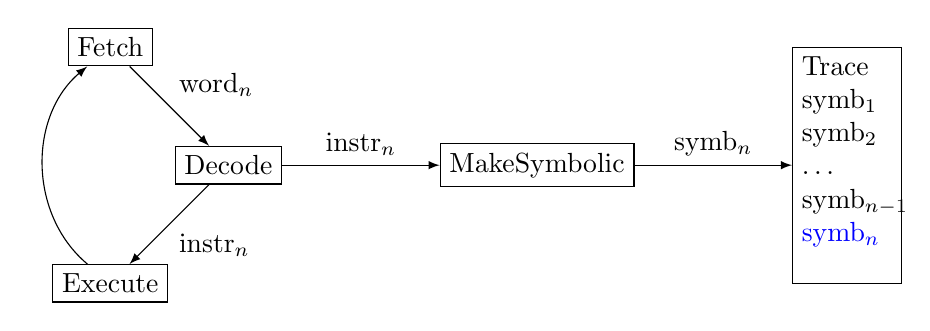
\begin{tikzpicture}[node distance = 1.5cm, auto]
\node [draw] (fetch) {Fetch};
\pause
\node [draw, below of=fetch, right of=fetch] (decode) {Decode};
\draw [-latex] (fetch) -- (decode) node [midway] {word$_n$};

\pause
\node [draw, below of=decode, left of=decode] (execute) {Execute};
\draw [-latex] (decode) -- (execute) node [midway] {instr$_n$};

\pause
\draw [-latex, bend left=50] (execute) edge (fetch);

\pause
\node [draw, right=2cm of decode] (symb) {MakeSymbolic};
\node [draw, right=2cm of symb, minimum height=3cm, text width=1.15cm] (trace) {};
\node [below right, text width=1cm] at (trace.north west) {Trace symb$_1$ symb$_2$ $\ldots$ symb$_{n - 1}$ \textcolor{blue}{symb$_n$}};
\pause

\draw [-latex] (decode) -- (symb) node [midway] {instr$_n$};
\pause
\draw [-latex] (symb) -- (trace) node [midway] {symb$_n$};
\end{tikzpicture}
\end{frame}

\begin{frame}{CPU (MakeSymbolic)}

\begin{tabular}{l | l}
Instruction & Symbolic \\
\hline
\pause
\lstinline{add $3, $1, $2} & $r_3 \gets r_1 + r_2$ \\
\pause
\lstinline{beq $1, $2, label} & $r_1 = r_2$ or $r_1 \neq r_2$ \\
\lstinline{add $3, $pc, $0} & $r_3 \gets \textsf{0x8BADF00D}$ \\
\lstinline{lis $3; 42} & $$ $r_3 \gets 42$
\end{tabular}
\end{frame}

\begin{frame}{Trace}
\begin{tikzpicture}[remember picture,overlay]
\node [draw] at (5,0) (trace) {Trace};
\node at (2, 0) (t) {$T$};
\node at (8, 0) (tp) {$T'$};

\draw [-latex] (t) -- (trace);
\draw [-latex] (trace) -- (tp);
\end{tikzpicture}

\pause
~\\
{\tt Seq[Trace => Trace]}
\pause
\begin{itemize}
\item Desugar
\pause
\item Simplify
\pause
\item Trim
\pause
\item SSA convert
\end{itemize}
\end{frame}

\begin{frame}[fragile]{Trace}
Desugar
\pause
\\
\lstinline{Mult(s, t)} $\rightarrow$ \lstinline{Mult64(tmp, s, t); Low32(lo, tmp); High32(hi, tmp)}
\pause
\\~\\
Simplify
\pause
\\
\lstinline{beq $0, $0, label} $\rightarrow \emptyset$ 
\pause
\\~\\
Trim
\\
\pause
limit trace to $D$ path conditions
\\~\\
\pause
SSA convert
\end{frame}

\begin{frame}{Trace (SSA convert)}

\begin{tabular}[fragile]{l | l | l}
Trace & Incorrect & Correct \\
\hline
\pause
\lstinline{Add(\$3, \$1, \$2)} & \pause $z = x + y$ & \pause $z_1 = x_1 + y_1$ \\
\pause
\lstinline{Sub(\$1, \$1, \$2)} & \pause $x = x - y$ & \pause $x_2 = x_1 - y_1$ \\
\pause
\lstinline{Add(\$2, \$1, \$2)} & \pause $y = x + y$ & \pause $y_2 = x_2 + y_1$
\end{tabular}
\pause
\\~\\`\\
$\$3 = 9 \land \$1 = 3$
\pause
\\
$z = 9 \land x = 3$
\pause
(no sol)
\\
\pause
$z_1 = 9 \land x_2 = 3$
\pause
$(x_1 = 6 \land y_1 = 3)$
\end{frame}

\end{document}